\documentclass[notitlepage,twocolumn,10pt]{article}

%\documentclass[notitlepage,10pt]{article}

\usepackage{nopageno}
\usepackage{amssymb}
%\usepackage[fleqn]{amsmath} % align all "\begin{equation} \end{equation}" sections to the left, more on alignment environments https://en.wikibooks.org/wiki/LaTeX/Advanced_Mathematics#Other_environments
\usepackage{amsmath}
\usepackage{graphicx}
\usepackage{float} % The "float" package is used to force figure positioning.
\usepackage{enumitem} % enriched labeled item

\usepackage{hyperref}
\graphicspath{ {./} } % Note that paths with underscore '_' or hyphen '-' should be avoided. 
\DeclareGraphicsExtensions{.pdf,.png,.jpg}

\usepackage{cleveref}
\crefname{enumi}{eq}{eqs} % reference "\item" as "\equation"

% set paragraph verticle spacing
\setlength{\parskip}{4.8pt}

\usepackage{titlesec}

\usepackage{mathrsfs}

% "style=numeric" is equivalent to "\bibliographystyle{unsrt}"
\usepackage[backend=bibtex,sorting=none,style=numeric]{biblatex}
\addbibresource{citations.bib} 

\titleformat{\section}[block]
  {\fontsize{12}{15}\bfseries\sffamily\filcenter}
  {\thesection}
  {1em}
  {\MakeUppercase}
\titleformat{\subsection}[hang]
  {\fontsize{12}{15}\bfseries\sffamily}
  {\thesubsection}
  {1em}
  {}

\begin{document}

% set verticle spacing for consecutive "\begin{equation} ... \end{equation}"s, should put AFTER "\begin{document}"
\abovedisplayskip=3pt
\abovedisplayshortskip=3pt
\belowdisplayskip=0pt
\belowdisplayshortskip=0pt
\abovecaptionskip=0pt
\belowcaptionskip=0pt

\title{Convex path planning and decoupled PID control for a powered descent landing problem}
\author{Yongfeng Lu, Zejian Chen}
\date{} % to remove the default date

\maketitle

\smallskip
%\small % use smaller font size, use "\footnotesize" for even smaller font
\footnotesize
\noindent \textbf{Abstract} A model-based path planning and control solution for the OpenAI/Gym Lunar Lander problem\cite{openaigym} is presented. The proposed approach uses the result of a convexified guidance path planning step to tune multiple decoupled PID controllers with feedforward routes. The approach is tested on a tailored OpenAI/Gym environment with more stringent or generalized constraints to demonstrate capability. 

\smallskip
\textbf{Keywords} convexification, socp, adaptive pid, feedforward, simulation  
\normalsize % recover normal font size

\section{Introduction} \label{sec:intro}
In \cite{openaigym} a Lunar Lander simulation environment was proposed, published solutions were mostly using reinforcement learning in either model-based or model-free manner\cite{yudeep, gadgil2020solving, peters2019dynamic}, hence an aim at feasibility of landing is often found as well as a lack of considerations for other realistic constraints such as landing site accuracy, fuel efficiency and movement speed. In this article a model-based landing approach on a tailored version of the OpenAI/Gym Lunar Lander is proposed, to show that the landing can be completed with several constraints including fuel and speed limits.      

\section{Problem Description} 

Given a lander with 2 engines from a starting position $\mathbf{r}_{0}$ in free fall state, we'd try to land it to the target position $\left( \begin{matrix} 0 \\ 0 \end{matrix} \right)$ while minimizing the speed upon landed.

\begin{figure}[H] % The "H" option comes from the "float" package.
    \centering
    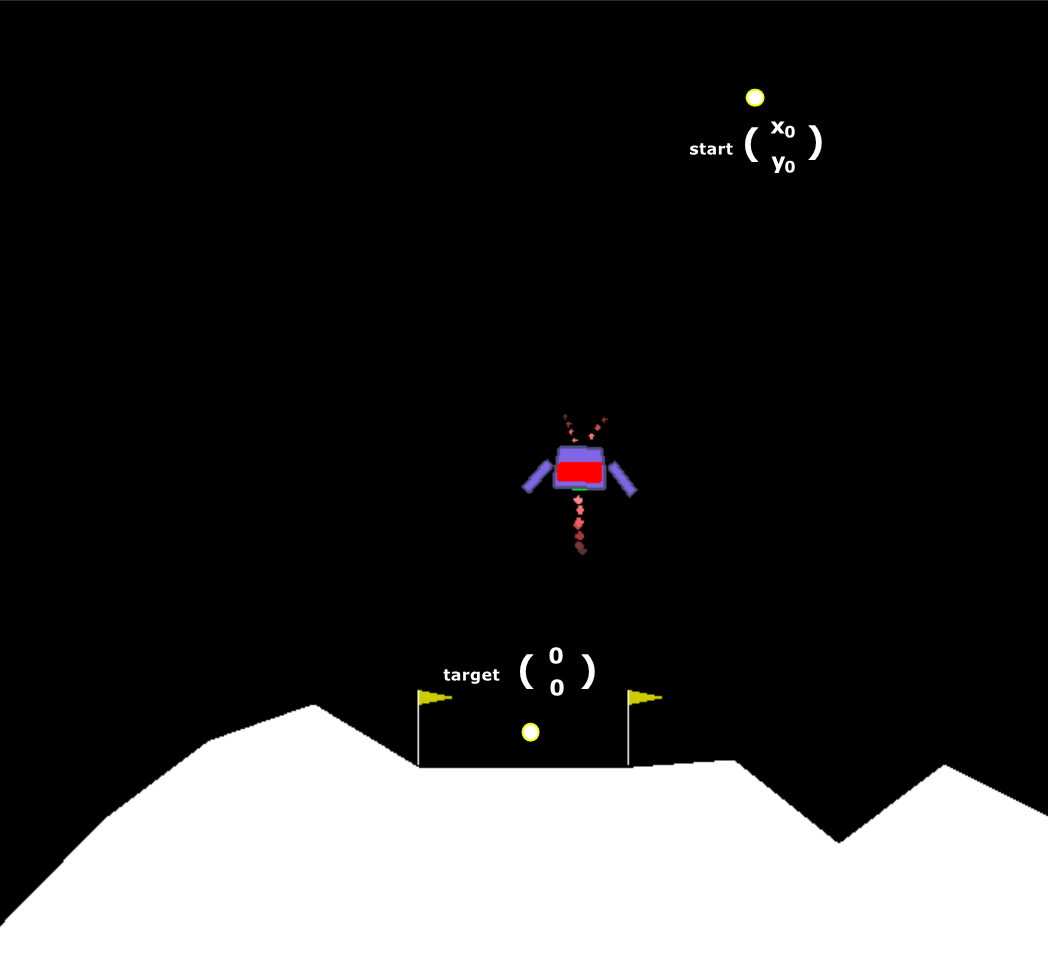
\includegraphics[width=8.0cm, keepaspectratio]{problem_desc}
    \caption{a lander to land on a target site by controlling engines}
    \label{fig:problem_desc}
\end{figure}

Kindly note that all variables in this article are assumed ``time varying'' if not otherwised declared to be constant.

The problem uses a lander(a.k.a. the ``plant'') which is simulated by Box2D physics engine and with the following components, yet the same approach can be generalized to 3D environment.
\begin{figure}[H] % The "H" option comes from the "float" package.
    \centering
    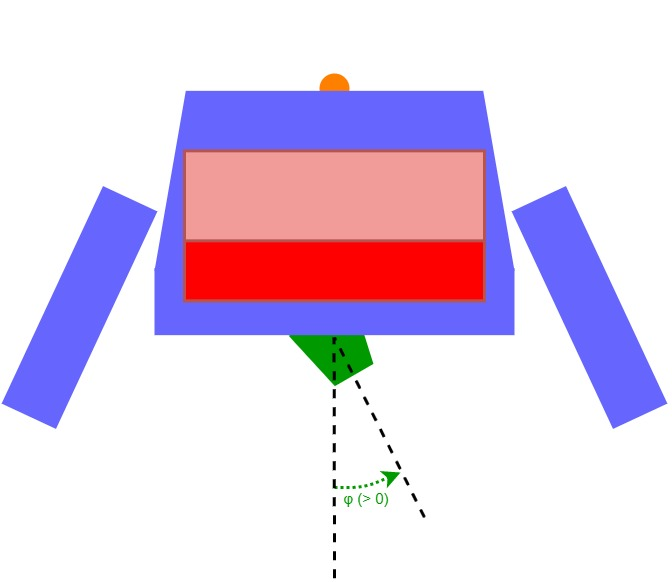
\includegraphics[width=4.0cm, keepaspectratio]{plant_geometry}
    \caption{2D plant with partially consumed fuel and gimbaled nozzle}
    \label{fig:plant_geometry}
\end{figure}

\begin{itemize}
    \item 1 near trapezoidal body that contributes to some of the total mass, the distance between the top edge and bottom edge is a constant $H$; the body mass is a constant $M_{b}$
    \item 2 massless legs attached to the body with revolute joints to provide support when landed
    \item 1 massless main thruster with gimbaled nozzle attached to the bottom of body, at any point of time the nozzle can gimbal at an angle $\phi \in [-\Phi_{max}, +\Phi_{max}] \; \& \; \Phi_{max} > 0$ w.r.t. the direction perpendicular to body top edge, and thrust magnitude $T_{b} \in [\rho_1, \rho_2] \; \& \; \rho_1, \rho_2 > 0$, the rate of change of each is unlimited
    \item 2 massless side thrusters attached to the top of body, at any point of time the net thrust $T_{s}$ is parallel to the direction parallel to body top edge, and constrained by $T_{s} \in ([-\rho_{side, 2}, -\rho_{side, 1}] \cup [\rho_{side, 1}, \rho_{side, 2}]) \; \& \; \rho_{side, 1} , \rho_{side, 2} > 0$ while the rate of change is unlimited, when $T_{s} > 0$ it's a net thrust to the right of the body top edge and $T_{s} < 0$ to the left
    \item 1 rectangular fuel tank inside the body that initially contributes to some of the total mass, when flying the fuel is consumed by a rate proportional to the thrusts, i.e. $\dot{m} = -\alpha \cdot (T_{b} + |T_{s}|)$ where $m$ is the total mass of the whole lander; the decrement of $m$ changes the overall center of mass during flight as well; the initial fuel mass is a constant $M_{f}$
\end{itemize}

The state-space measurement $\mathbf{q}$ and maneuver $\mathbf{w}$ of this ``plant'' are denoted as follows.
\begin{equation} \label{eqs:state}
\mathbf{q} \, := \left( \begin{matrix} \mathbf{r} \;\, \dot{\mathbf{r}} \;\, \theta \;\, \dot{\theta} \;\, m \;\, \dot{m} \end{matrix} \right)^T
\end{equation}
\begin{equation} \label{eqs:maneuver}
\mathbf{w} \, := \left( \begin{matrix} T_{b} \;\, \phi \;\, T_{s} \end{matrix} \right)^T
\end{equation}


There is no wind dynamics in this problem, yet later in \cref{sec:gdc} the planned path can be constrained to low speed for alleviating impact if necessary.

\section{Model Description and Estimations}

\begin{figure}[H] % The "H" option comes from the "float" package.
    \centering
    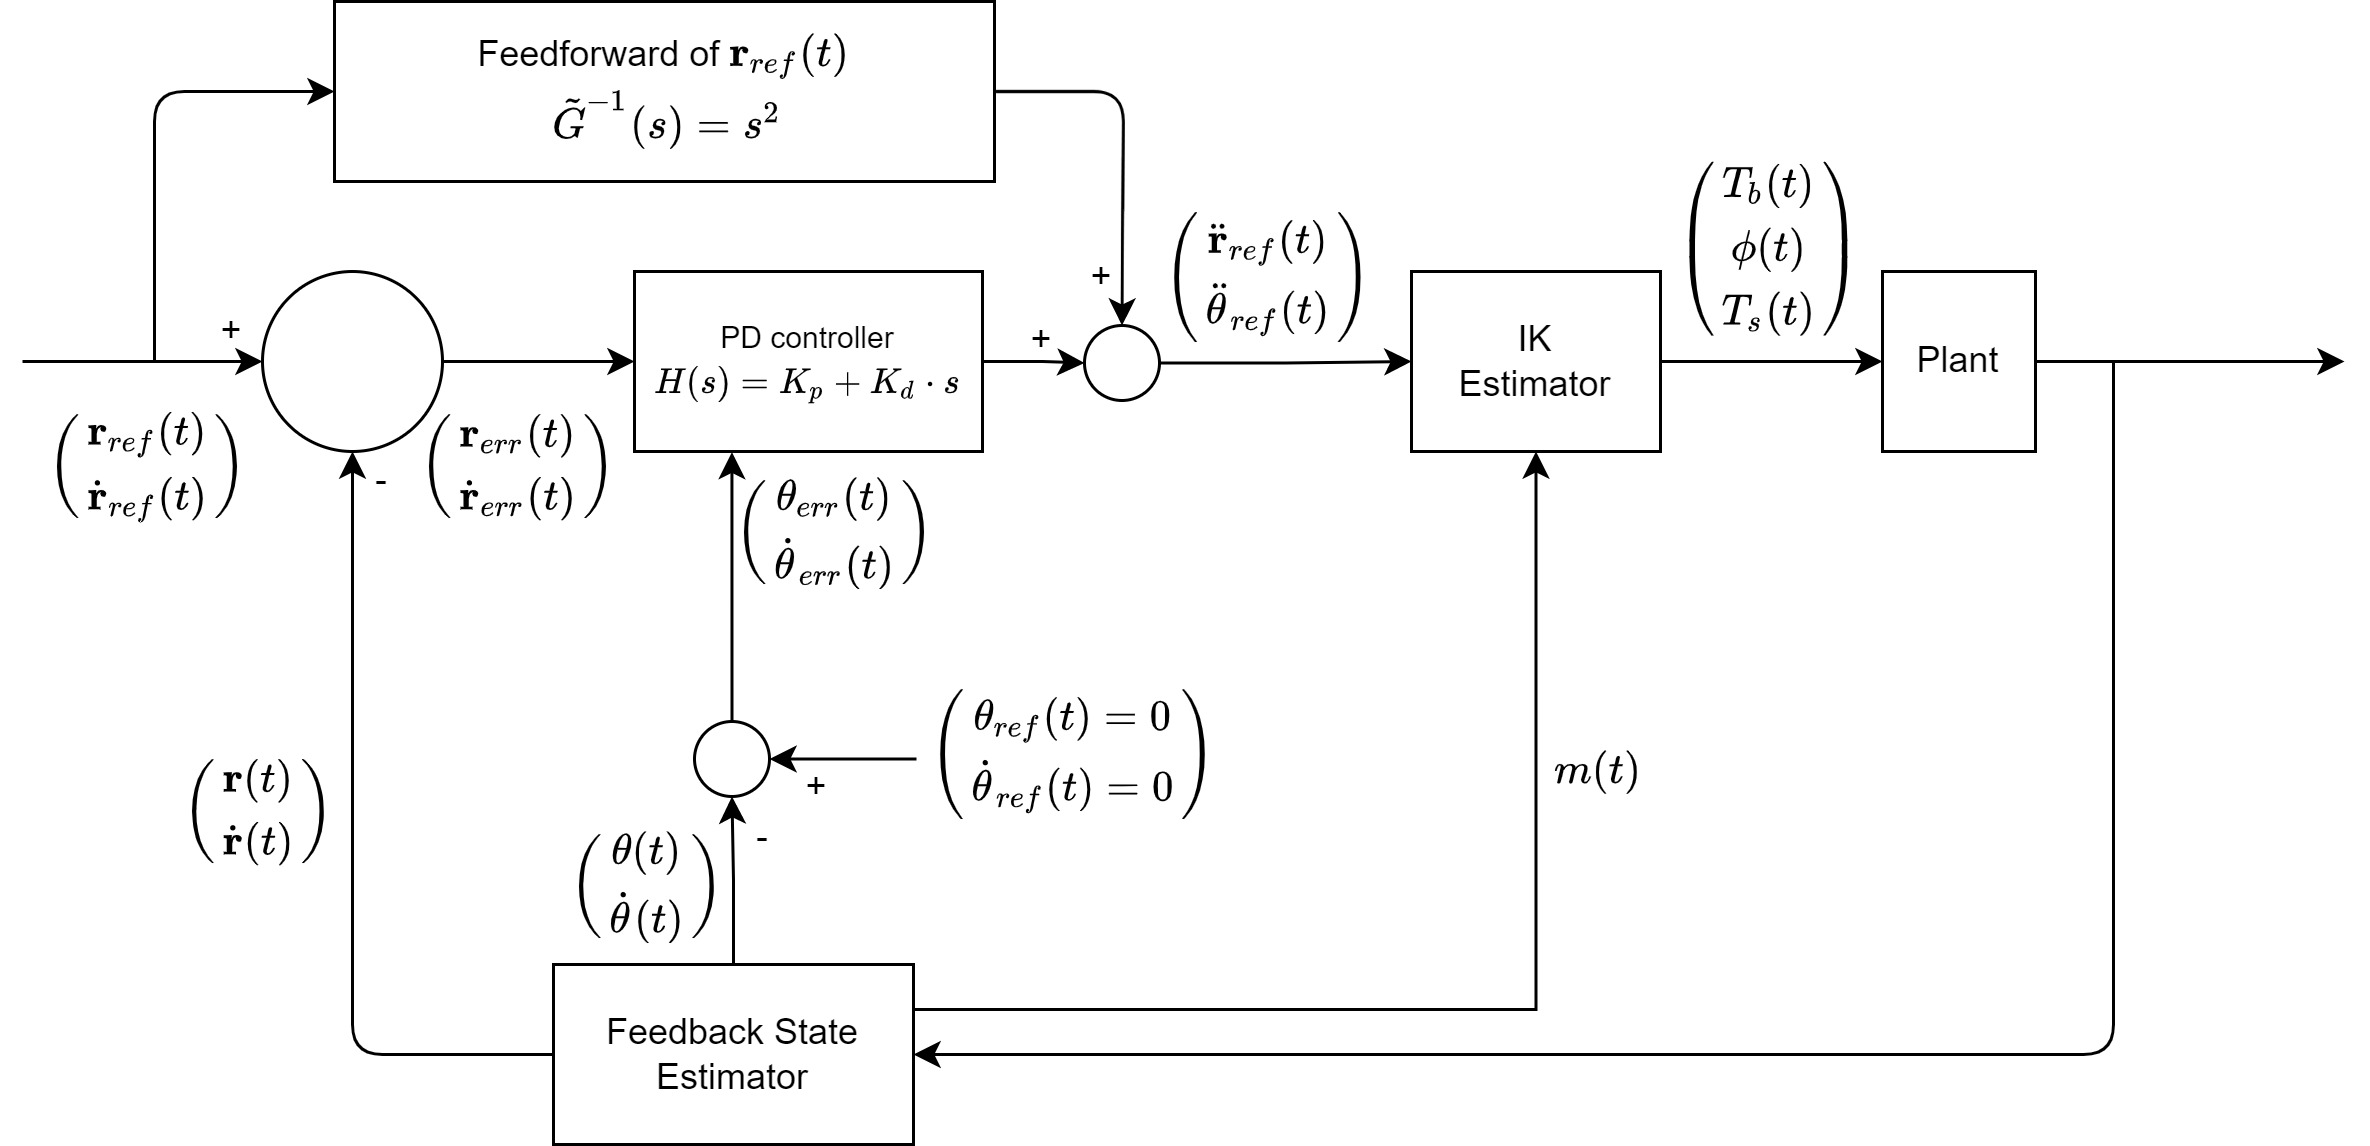
\includegraphics[width=9.0cm, keepaspectratio]{PD_feedforward_block}
    \caption{Block diagram of controller}
    \label{fig:PD_feedforward_block}
\end{figure}

The solution assumes that we can obtain the following feedback states of the ``plant''.
\begin{enumerate}[label=\textbf{a.\arabic*}, itemsep=2pt] % or "nosep" in the place of "itemsep=..." to make even less vspace
  \item \label{eqs:r} $\begin{pmatrix} \mathbf{r} \\ \dot{\mathbf{r}} \end{pmatrix}$, position and velocity of the body 
  \item \label{eqs:theta} $\begin{pmatrix} \theta \\ \dot{\theta} \end{pmatrix}$, tilted angle of the body w.r.t. y-axis and angular velocity w.r.t. the axis perpendicular to center of mass of the body alone
  \item \label{eqs:m} $m$, total mass of the whole lander
\end{enumerate}

\begin{figure}[H] % The "H" option comes from the "float" package.
    \centering
    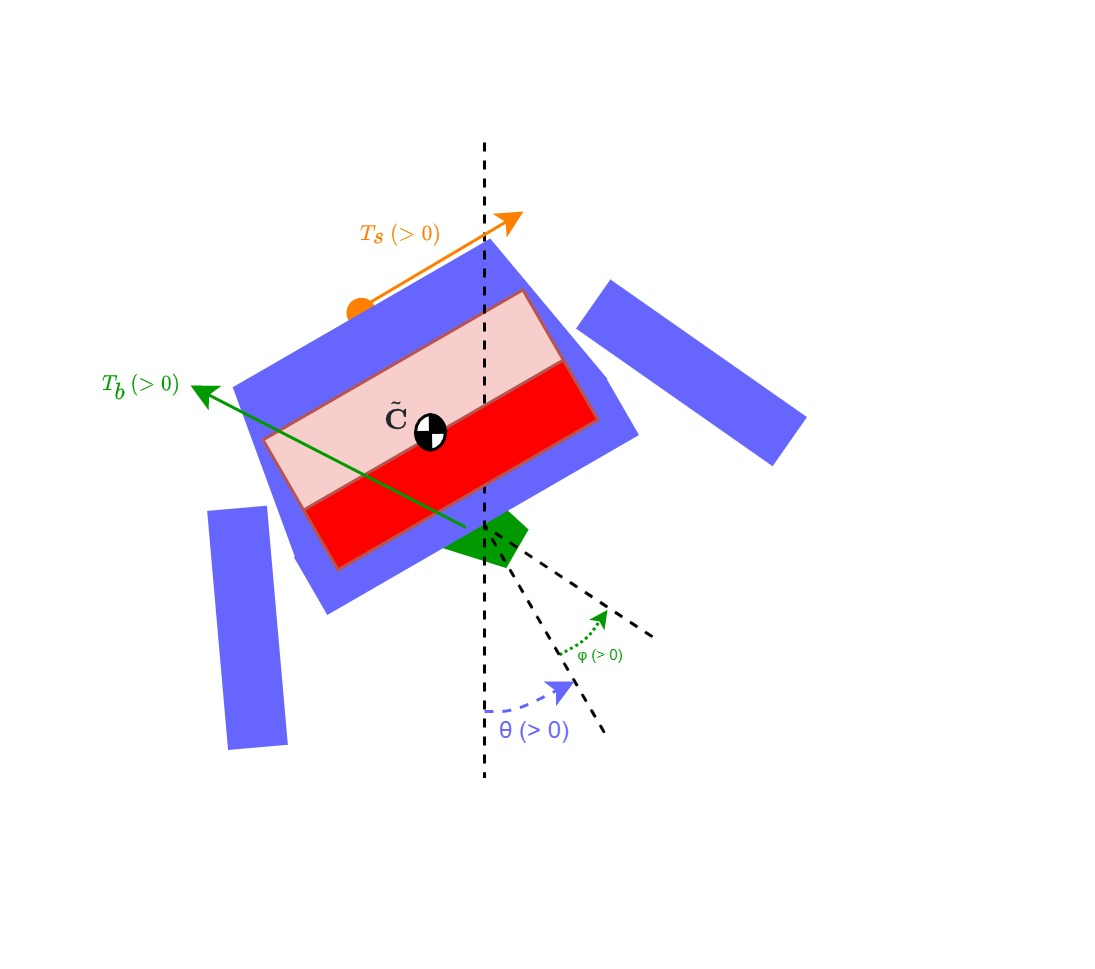
\includegraphics[width=7.0cm, keepaspectratio]{model_forces}
    \caption{Modeled forces of the plant}
    \label{fig:model_forces}
\end{figure}

In \cref{fig:PD_feedforward_block} the ``IK(Inverse Kinematics) Estimator'' will take the following estimations to simplify the model.
\begin{enumerate}[label=\textbf{b.\arabic*}, itemsep=2pt]
    \item \label{eqs:C} $\tilde{\mathbf{C}}$, the estimated overall center of mass of the lander, which sits in the exact middle of the segment between the mid-point of body top edge and mid-point of body bottom edge, i.e. a constant position at all time
    \item \label{eqs:Iz} $\tilde{I_z} = m \cdot (\frac{H}{2})^2$, estimated magnitude of angular moment of inertia of the whole lander w.r.t. line parallel to z-axis through $\tilde{\mathbf{C}}$
\end{enumerate}

Therefore the estimated dynamics would be

\begin{equation} \label{eqs:accLinear}
\ddot{\mathbf{r}} \cdot m= \begin{pmatrix}
    -sin(\theta + \phi) & cos\theta \\
    cos(\theta + \phi) & sin\theta
\end{pmatrix} \cdot \begin{pmatrix}
  T_{b} \\
  T_{s} 
\end{pmatrix} + \begin{pmatrix} 
    0 \\
    - g \cdot m
\end{pmatrix}
\end{equation}

\begin{equation} \label{eqs:accIznewton}
\ddot{\theta} \cdot \tilde{I_z} = T_{b} \cdot sin\phi \cdot \frac{H}{2} + T_{s} \cdot \frac{H}{2}
\end{equation}

It'll soon be shown that such simplification of $\tilde{I_z}$ fits the controller well. Moreover, this estimation approach is convenient to be applied to 3D case as well. 


\section{Guidance and Control} \label{sec:gdc}
\subsection{Guidance planning} \label{sec:gdp}

The guidance algorithm here aims at finding a solution $(\mathbf{r_{ref}}, \dot{\mathbf{r}}_{ref})$ to the problem while trying to minimize the total fuel consumption.

Denote that  

$\mathbf{F} \, := \left( \begin{matrix}
    -sin(\theta + \phi) & cos\theta \\
    cos(\theta + \phi) & sin\theta
\end{matrix} \right) \cdot \left( \begin{matrix}
  T_{b} \\
  T_{s} 
\end{matrix} \right)$ 

being the total force from engines, we can rephrase the problem with minimal fuel goal to the following.

\textbf{Problem 1 (non-convex)}

$\underset{t_f, \mathbf{F}}{\max} \; \tilde{m}(t_f) = \underset{t_f, \mathbf{F}}{\min} \int_{0}^{t_f} ||\mathbf{F}|| \cdot dt$

where
\begin{equation*}
\tilde{m}(0) = M_{b} + M_{f}
\end{equation*}
\begin{equation*}
\dot{\tilde{m}} = -\alpha \cdot ||\mathbf{F}||
\end{equation*}
\begin{equation*} \label{eqs:esrho}
\tilde{\rho}_1 \le ||\mathbf{F}|| \le \tilde{\rho}_2 
\end{equation*}
\begin{equation*}
\mathbf{r}(t_f) = \dot{\mathbf{r}}(t_f) = \dot{\mathbf{r}}(0) = \begin{pmatrix} 0 \\ 0 \end{pmatrix}
\end{equation*}
\begin{equation*}
\mathbf{r}(0) = given \, start \, position
\end{equation*}
\begin{equation*}
\ddot{\mathbf{r}} = \frac{\mathbf{F}}{\tilde{m}} + \begin{pmatrix} 0 \\ - g \end{pmatrix}
\end{equation*}
\begin{equation*}
\tilde{m}(t_f) \ge M_b + (1 - \lambda) \cdot M_f
\end{equation*}
\begin{equation*} 
\mathbf{r}_1 \ge 0 
\end{equation*}

Kindly note there's an empirically chosen constant $\lambda$, and an estimation $\tilde{m}$ instead of $m$ is used here because in general $\dot{\tilde{m}} \le \dot{m}$, thus we can be more conservative to constrain that $\lambda \le 0.7$, i.e. plan to use only up to $70\%$ of the fuel. 

The new thrust bounds $\tilde{\rho}_1, \tilde{\rho}_2$ could've been estimated from $\rho_1, \rho_2, \rho_{side,1}, \rho_{side,2}, \Phi_{min}, \Phi_{max}$ analytically, but in practice it's fair to just take the following approximations because we expect the main engine to contribute most to the thrust magnitude.
\begin{equation*} \label{eqs:esrhoapprox}
\tilde{\rho}_1 = \rho_1, \; \tilde{\rho}_2 = \rho_2
\end{equation*}


According to \cite{cvxpow, losslesscvx} Problem 1 is non-convex but can be losslessly convexified to the following SOCP\cite{alizadeh2003second}.

\textbf{Problem 2 (SOCP)}

$\underset{t_f, \mathbf{u}, \sigma}{\min} \; \int_{0}^{t_f} \sigma \cdot dt$

where 
\begin{equation}
\eta(0) = \ln(M_{b} + M_{f})
\end{equation}
\begin{equation}
\mathbf{r}(t_f) = \dot{\mathbf{r}}(t_f) = \dot{\mathbf{r}}(0) = \begin{pmatrix} 0 \\ 0 \end{pmatrix}
\end{equation}
\begin{equation}
\mathbf{r}(0) = given \, start \, position
\end{equation}
\begin{equation}
\ddot{\mathbf{r}} = \mathbf{u} + \begin{pmatrix} 0 \\ -g \end{pmatrix}
\end{equation}
\begin{equation} \mu_1 (1-(\eta-\eta_0)+\frac{(\eta-\eta_0)^2}{2}) \le \sigma \le \mu_2 (1-(\eta-\eta_0)) \end{equation}
\begin{equation}
\eta_0 \le \eta \le \ln(M_b + M_f - \alpha \cdot \tilde{\rho}_1 \cdot t)
\end{equation}
\begin{equation} ||\mathbf{u}|| \le \sigma \end{equation}
\begin{equation} \dot{\eta} = -\alpha \cdot \sigma \end{equation}
\begin{equation}
\eta(t_f) \ge \ln(M_b + (1 - \lambda) \cdot M_f)
\end{equation}
\begin{equation} 
\mathbf{r}_1 \ge 0 
\end{equation}

by introducing new variables
\begin{equation*} \label{eqs:slacku}
\mathbf{u} \, := \frac{\mathbf{F}}{\tilde{m}}
\end{equation*}
\begin{equation*} \label{eqs:slacketa}
\eta \, := \ln(\tilde{m})
\end{equation*}
\begin{equation*} \label{eqs:eta0}
\eta_0 \, := \ln(M_b + M_f - \alpha \cdot \tilde{\rho}_2 \cdot t)
\end{equation*}
\begin{equation*} \label{eqs:mu}
\mu_1 \, := \tilde{\rho}_1 \cdot e^{-\eta_0}, \mu_2 = \tilde{\rho}_2 \cdot e^{-\eta_0}
\end{equation*}

The following ``low speed'' constraints can be added to Problem 2 without breaking the SOCP compliance.  
\begin{equation} 
\dot{\mathbf{r}}_1 \le given \, descending \, speed \, limit
\end{equation}
\begin{equation} 
|\ddot{\mathbf{r}}_1| \le given \, descending \, acceleration \, limit
\end{equation}

When given a certain termination time-of-flight $t_f$ and discretized about $t$, Problem 2 can be numerically solved in an efficient manner by using SOCP specific solvers like ECOS\cite{domahidi2013ecos}. The search for a feasible $t_f$ will be in range $t_f \in [\frac{M_b \cdot |\dot{\mathbf{r}}(0)|}{\rho_2}, \frac{M_f}{\rho_1}]$

\subsection{Controller design}

Given $\begin{pmatrix} \mathbf{r}_{ref} \\ \dot{\mathbf{r}}_{ref} \end{pmatrix}$, a controller is needed to track the reference path. 

The \cref{eqs:accLinear,eqs:accIznewton} w.r.t. \cref{eqs:state} \& \cref{eqs:maneuver} forms a Multi Input Multi Output (MIMO) system, an intuitive choice would be to obtain a linearized $\frac{d\mathbf{q}}{dt} = \mathbf{A} \cdot \mathbf{q} + \mathbf{B} \cdot \mathbf{w}$ from \cref{eqs:accLinear,eqs:accIznewton} at a chosen trim point, then apply a Model Predictive Control by scoring proximity to $\begin{pmatrix} \mathbf{r}_{ref} \\ \dot{\mathbf{r}}_{ref} \end{pmatrix}$. 

However there's inconvenience for linearizing this model. Only part of $\mathbf{q}$ can be linearized because $\dot{m} \ne 0$ during flight, and a non-hover flight might remove $\left( \mathbf{r} \;\, \dot{\mathbf{r}} \right)$ from linearizable parts over all time\cite{kim2020modeling}, resulting in extra complications in design of the whole controller as the non-linearized parts are not decoupled.     

For this problem the relatively simple PID controllers with the non-linear model suffices to work to satisfaction. By decoupling inputs and outputs into several SISO PID controllers, we avoid empirically guessing any cross coupled factors for \cref{eqs:maneuver} w.r.t. \cref{eqs:r,eqs:theta,eqs:m}, as shown in the figure below.

\begin{figure}[H] % The "H" option comes from the "float" package.
    \centering
    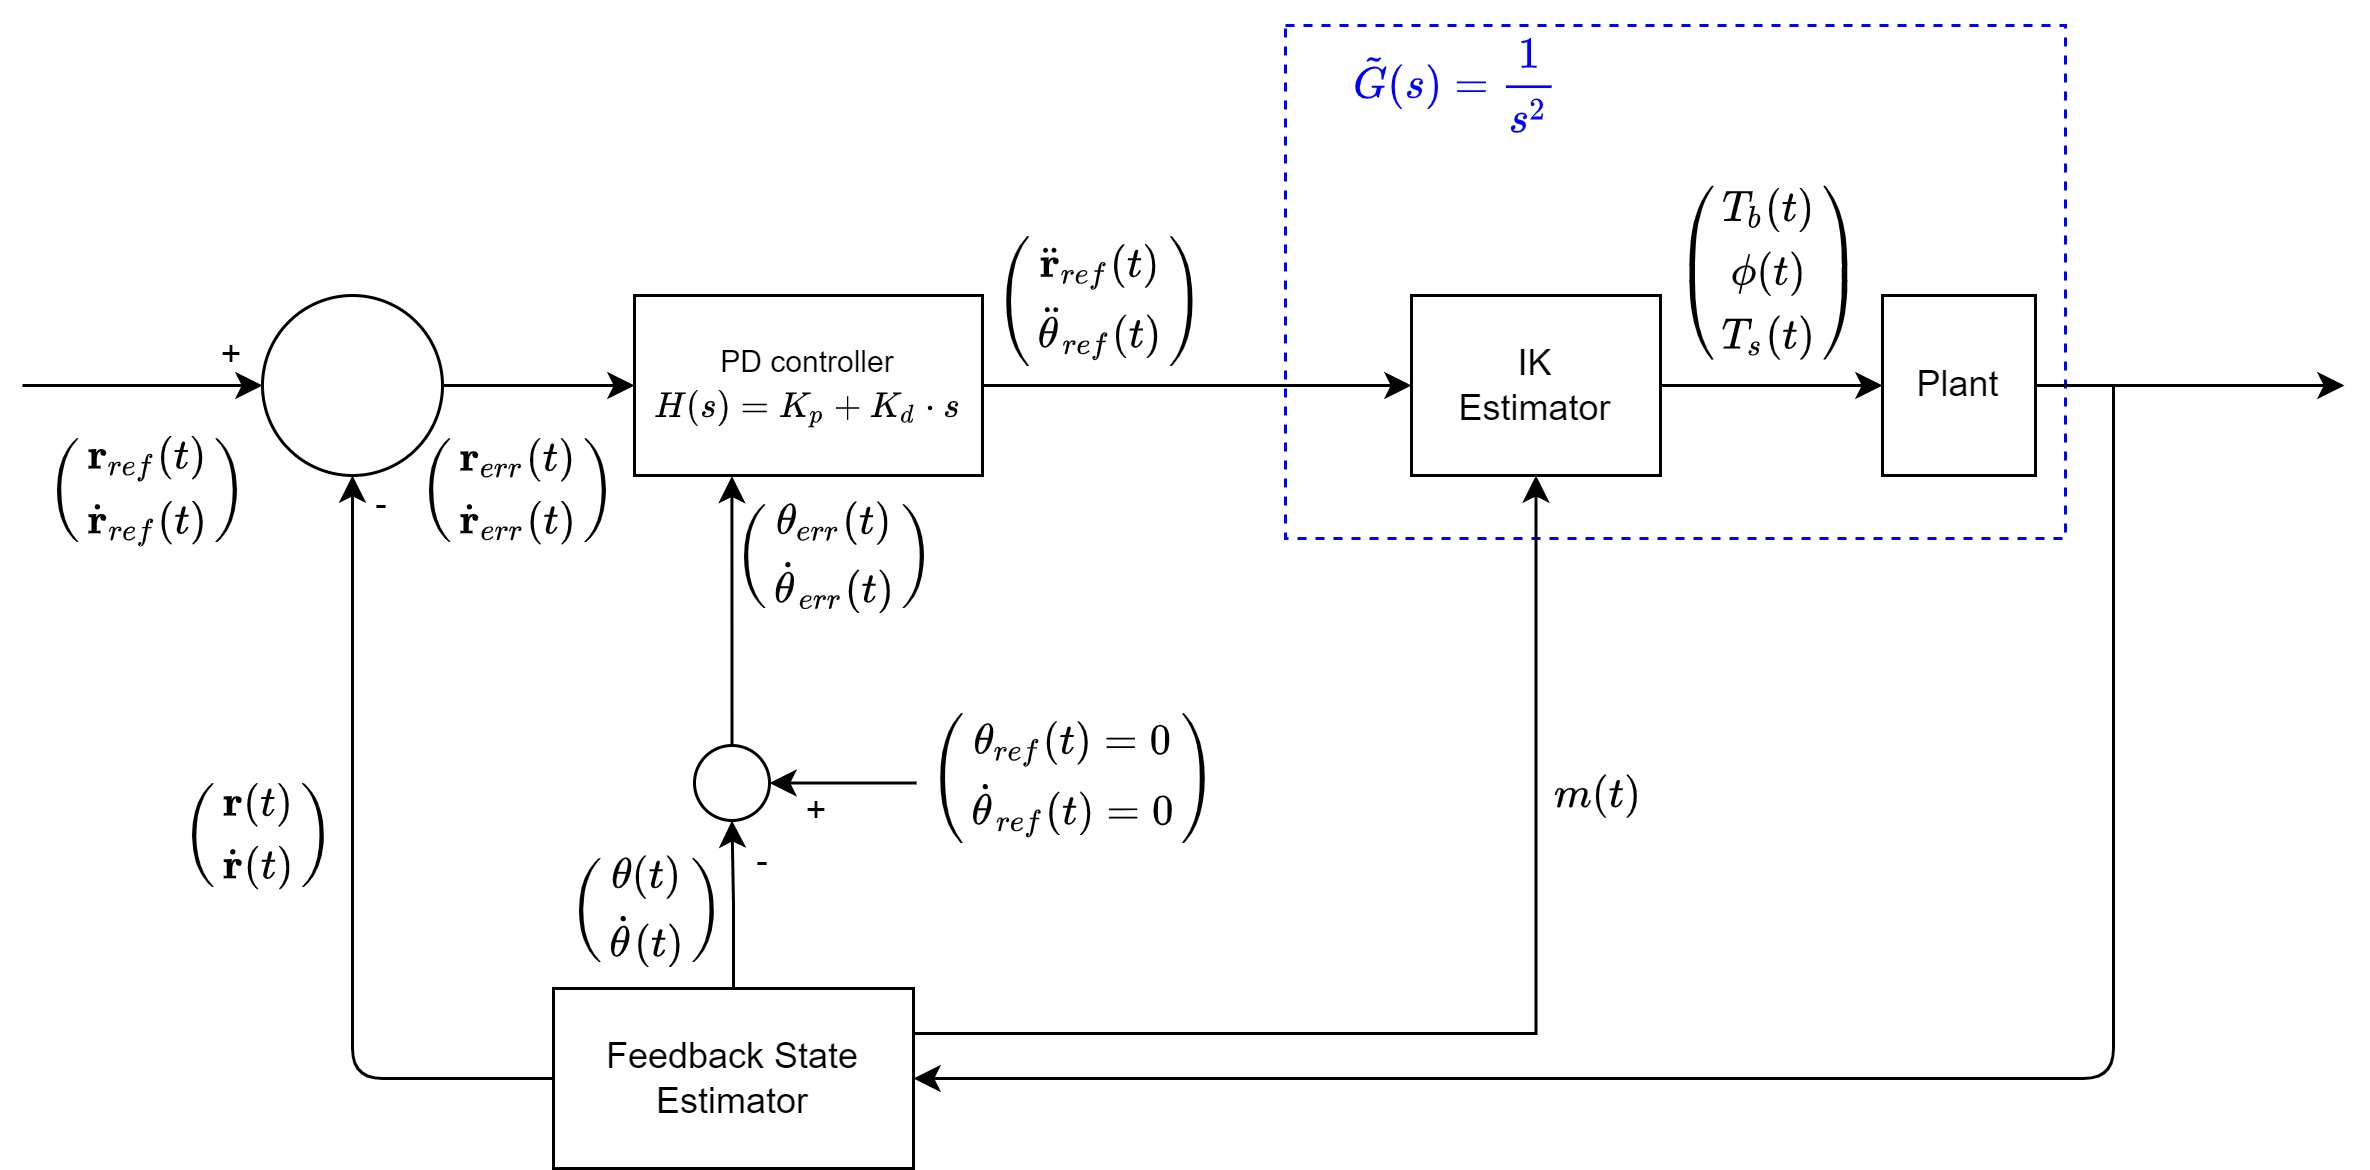
\includegraphics[width=9.0cm, keepaspectratio]{PD_block}
    \caption{Block diagram of non-feedforward controller}
    \label{fig:PD_block}
\end{figure}

First, each of the SISO PID controller would be just a classical PD controller and only responsible for single dimensional position or rotation control, i.e. w.r.t. one of x-axis, y-axis and z-axis
\begin{equation} \label{eqs:Gtilde}
\tilde{G}(s) = \frac{1}{s^2}
\end{equation}
\begin{equation} \label{eqs:Hr}
H_{\mathbf{r}}(s) = K_{p,\mathbf{r}} + s \cdot K_{d,\mathbf{r}} 
\end{equation}
\begin{equation} \label{eqs:Htheta}
H_{\theta}(s) = K_{p,\theta} + s \cdot K_{d,\theta}
\end{equation}
\begin{equation} \label{eqs:closedlooptf1}
\mathcal{L}\{ \mathbf{r} \}= \frac{\tilde{G} \cdot H_{\mathbf{r}}}{1 + \tilde{G} \cdot H_{\mathbf{r}}} \cdot \mathcal{L}\{ \mathbf{r}_{ref} \}
\end{equation}
\begin{equation} \label{eqs:closedlooptf2}
\mathcal{L}\{ \theta \}= \frac{\tilde{G} \cdot H_{\theta}}{1 + \tilde{G} \cdot H_{\theta}} \cdot \mathcal{L}\{ \theta_{ref} \}
\end{equation}

where $\mathcal{L}\{\cdot\}$ indicates the Laplace transform. 

The $\sim$ on \cref{eqs:Gtilde} means that it's an estimation that the ``IK Estimator'' and ``Plant'' steps can achieve
\begin{equation*}
\begin{pmatrix} \mathbf{r}(t) \\ \theta(t) \end{pmatrix} = \int_0^t \begin{pmatrix} \ddot{\mathbf{r}}_{ref}(\tau) \\ \ddot{\theta}_{ref}(\tau) \end{pmatrix} \cdot d \tau
\end{equation*}
in good fidelity. 

That \cref{eqs:Gtilde} being a ``no delay \& no damp double integrating'' transfer function makes it a peculiar second order system to design the PID controller. In a wellknown case    
\begin{equation} \label{GtildeAlt}
  \tilde{G}_{alt}(s) = \frac{e^{-\gamma s}}{(\delta_1 s + 1)(\delta_2  s + 1)}
\end{equation}
, simple IMC approach to estimate $2^{nd}$-order approximator and then a single parameter tunable PID controller is proposed in \cite{skogestad2012simc}. However in a simulation environment without air dynamics, \cref{eqs:Gtilde} will remain as-is and thus even the treatments in \cite{grimholt2016optimal, ruscio2017tuning} wouldn't be applicable due to $\gamma = 0$. 

Aiming at an analytical approach to determine the variables in \cref{eqs:Hr,eqs:Htheta} and knowing that derivative action is necessary for stabilization for \cref{eqs:Gtilde}\cite{grimholt2016optimal}, every PID controller is limited to be a PD controller in our approach and the steady state error will instead be complemented by a feedforward route. 

In the context of this paper, we're only concerned with a single $\theta$ and the control of $\theta$ should favor a small peak overshoot, therefore both $K_{p, \theta}$ and $K_{d, \theta}$ in \cref{eqs:Htheta} will be chosen as constants in \cref{sec:const}.

To compute proper $K_{p, \mathbf{r}}$ and $K_{d, \mathbf{r}}$, as we're also constrained by 
$T_{settle} < t_f$ from the \cref{sec:gdp}, an analytical $\tilde{T}_{settle}(K_p, K_d)$ for each dimension is preferrable given requirements of the unit step response of \cref{eqs:closedlooptf1} 
\begin{enumerate}[label=\textbf{c.\arabic*}, itemsep=2pt]
    \item \label{eqs:setrange} $SettlingTimeThreshold = 0.05$    
    \item \label{eqs:pOS} $PeakOvershoot_0 = 0.15$
    \item \label{eqs:Tsettle} $\tilde{T}_{settle, 0} = (0.6 \cdot t_f)$, the intersection of amplitude envelope of $\mathcal{L}^{-1}\{\frac{\tilde{G} \cdot H_{\mathbf{r}}}{1 + \tilde{G} \cdot H_{\mathbf{r}}} \cdot \frac{1}{s}\}$ and the $SettlingTimeThreshold$ horizon
\end{enumerate}
, to numerically find a fit for both
\begin{enumerate}[label=\textbf{d.\arabic*}, itemsep=2pt]
    \item $|\frac{\tilde{T}_{settle}(K_{p,\mathbf{r}}, \, K_{d,\mathbf{r}})}{\tilde{T}_{settle, 0}} - 1| < 0.05$, and
    \item $|\frac{PeakOvershoot(K_{p,\mathbf{r}}, \, K_{d,\mathbf{r}})}{PeakOvershoot_0} - 1| < 0.05$
\end{enumerate}
, where the analytical form of $\tilde{T}_{settle}(\cdot, \cdot)$ and $PeakOvershoot(\cdot, \cdot)$ can be calculated by symbolic calculation tools. 

Next, Given a $\ddot{\mathbf{r}}_{ref}$ computed by the ``PD Controller'' step, the ``IK Estimator'' computes \cref{eqs:maneuver} numerically from \cref{eqs:accLinear,eqs:accIznewton}.

Lastly, the ``Plant'' in simulation will guarantee to clip $T_{b} \in [\rho_1, \rho_2]$, $\phi \in [-\Phi_{max}, +\Phi_{max}]$ and $T_{s} \in ([-\rho_{side, 2}, -\rho_{side, 1}] \cup [\rho_{side, 1}, \rho_{side, 2}])$ before stepping in the physics engine.

Kindly note that compared to \cref{fig:PD_block}, \cref{fig:PD_feedforward_block} adds a feedforward route $\tilde{G}^{-1}(s) = s^2$ which reduces delay in $\dot{\mathbf{r}}$ tracking $\dot{\mathbf{r}}_{ref}$\cite{visioli2004new}.

\section{Simulation Results}
\subsection{Constants} \label{sec:const}

All using SI units and referencing the Masten XL-1 mass profile.
\begin{equation*}
|g| = 9.81 \, m^2/s, \, \text{same gravity as the earth}
\end{equation*}
\begin{equation*}
H = 27 \, m, \, M_b = 728.28 \, kg, \, M_f = 1699.32 \, kg
\end{equation*}
\begin{equation*} 
\Phi_{max} = 0.087 \, rad, \, \alpha = 0.0015 \, \frac{kg}{s \cdot N}
\end{equation*}
\begin{equation*} 
\rho_1 = 7282.8 \, N, \, \rho_2 = 24276.0 \, N
\end{equation*}
\begin{equation*} 
\rho_{side,1} = 728.28 \, N, \, \rho_{side,2} = 2427.6 \, N
\end{equation*}
\begin{equation*}
\text{guidance discretization fps} =  15 \, frames/s
\end{equation*}
\begin{equation*}
\text{simulation \& renderer fps} =  60 \, frames/s
\end{equation*}
\begin{equation*}
K_{p, \theta} = 131.1244, \, K_{d, \theta} = 21.175025483564053
\end{equation*}
\begin{equation*}
(PeakOvershoot = 0.05, \, T_{settle} = 0.5 \, s)
\end{equation*}

\subsection{Results}
TBD.

6 starting positions, each with 50 episodes with planned-actual deviation stats.

for each starting position

measured v.s. planned

- $t_f$ (diff in \%)
  
  - - computed $K_{p, \mathbf{r}}$ and $K_{d, \mathbf{r}}$

- landing mass (diff in \%)

- landing position (diff in \%)

- landing velocity (diff in \%)

\section{Conclusion}
The guided path can be tracked pretty well by the PD controllers with ``IK Estimator'' regardless of the rotational dynamics not respected in \cref{sec:gdp}.

The approach here is deterministic, capable of not only landing the plant but also imposing practical constraints such as descending speed, gliding cone space etc. on the path. As each PD controller is mutually independent, it can be generalized to 3D environment with minor changes to the ``IK Estimator''. 

Further development of the approach should take re-ignition cost and limitations into account, as not all engines are designed re-ignitable or can be re-ignited for an unlimited number of times\cite{sutton2006history,zhao2016real}.    

\printbibliography

\end{document}
